�реключения состояния обслуживающего устройства. Определим следующие случайные величины и элементы:
\begin{itemize}
\item количество $\vk_{j,i} \in Z_+ $ требований в очереди $O_j$ в момент времени $\tau_i$;
\item состояние обслуживающего устройства $\G_i\in \G = \brrr{\G^{(1)},\G^{(2)}, \ldots, \G^{(n)}}$ в течение $\left(\tau_{i-1};\tau_i\right]$;
\item количество $\eta_{j,i}$ требований, поступивших в очередь $O_j$ по потоку $\Pi_j$ в течение $\left(\tau_{i};\tau_{i+1}\right]$;
\item количество $\xi_{j,i}$ требований по потоку насыщения $\Pi^{\mathrm{sat}}_j$ в течение $\left(\tau_{i};\tau_{i+1}\right]$;
\item количество $\overline{\xi_{j,i}}$ реально обслуженных требований по потоку $\Pi_j$,
\end{itemize}
для $j=\overline{1,4}$.






В данной работе будет применен так называемый кибернетический подход, который предполагает, что наблюдение за системой осуществляется в дискретные моменты времени $\tau_0 = 0,~ \tau_1,~ \ldots$,~  совпадающие с моментами переключения состояния обслуживающего устройства. 
Будем считать, что функция перехода из состояния $\G_i$ в момент $\tau_i$ в состояние $\G_{i+1}$ в момент $\tau_{i+1}$ известна и задается функцией $h(\G_i,x_i)$ от предыдущего состояния $\G_i$ и величины $x_i$ очереди $O_3$ в момент $\tau_i$. Таким образом, обслуживающее устройство, в зависимости от объема очереди $O_3$, может переходить в разные состояния, что влечет за собой особый класс рассматриваемых графов переходов. Опишем сейчас общую структуру класса ${\cal K}$ рассматриваемых графов переходов между состояниями обслуживающего устройства (ОУ).

Первое и самое очевидное требование, которое мы наложим на рассматриваемый класс графов, --- это ориентированность и связность. Порядок прохождения состояний ОУ имеет значение и рассматривать недостижимые состояния (которые делают граф несвязным) не имеет смысла.

Далее, будем предполагать, что каждый граф $G$ из класса ${\cal K}$ может быть построен по следующему алгоритму.
\begin{enumerate}
\item Выделить из множества всех вершин графа $d$ непересекающихся кластеров вершин $C_1$, $C_2$, $\ldots$, $C_d$ таким образом, чтобы вершины внутри кластеров были соединены в цикл. Каждый кластер $C_j$ в свою очередь разделить на три непересекающихся множества вершин $C_j=C_j^{\mathrm{I}} + C_j^{\mathrm{O}} + C_j^{\mathrm{N}}$. Множество $C_j^{\mathrm{I}}$ будем называть множеством входных вершин, $C_j^{\mathrm{O}}$~--- множеством выходных вершин и $C_j^{\mathrm{N}}$~--- множеством нейтральных вершин. (Рис.~\ref{GraphSchemeOne}).

\begin{figure}[h]
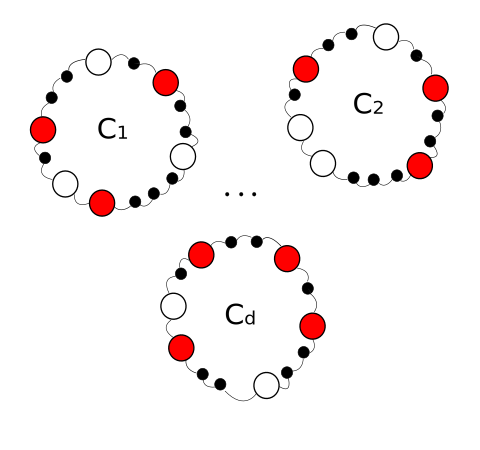
\includegraphics[scale=0.4]{GraphScheme1.png} 
\caption{Класс графов переходов (Шаг 1). Незакрашенные вершины --- выходные вершины, красным отмечены входные вершины, черным --- нейтральные}
\label{GraphSchemeOne}
\end{figure}
\item Каждое выходное состояние $c_1$ некоего кластера $C_j$ может быть соединено с входным состоянием того же или другого кластера $C_k$ постредством сторонней вершины $c$, не принадлежащей никакому из кластеров $C_1$, $C_2$, $\ldots$, $C_d$, и двух соединящих ребер (Рис.~\ref{GraphSchemeTwo}).
\begin{figure}[h]
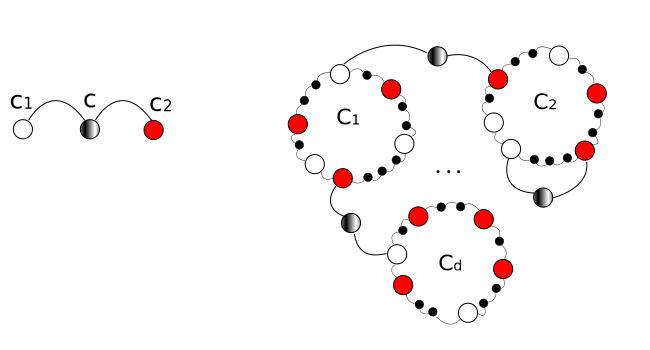
\includegraphics[scale=0.4]{GraphScheme2.png} 
\caption{Класс графов переходов (Шаг 2). Слева~--- шаблон соединения выходной и входной вершин. Справа~--- пример получаемого графа после шага 2. Полузакрашенные вершины~--- сторонние вершины, не принадлежащие ни одному кластеру $C_1$, $C_2$, $\ldots$ $C_d$}
\label{GraphSchemeTwo}
\end{figure}

\item Каждая сторонняя вершина, получаемая на шаге $2$, может быть соединена похожим образом с входной вершиной некоего кластера $C_j$: то есть посредством новой (еще не учавствовавшей в построении графа) сторонней вершины и двух новых ребер, или же посредством уже существующей сторонней (не входящей ни в один из кластеров) вершины и всего одного нового ребра (Рис.~\ref{GraphSchemeTree}).

\begin{figure}[h]
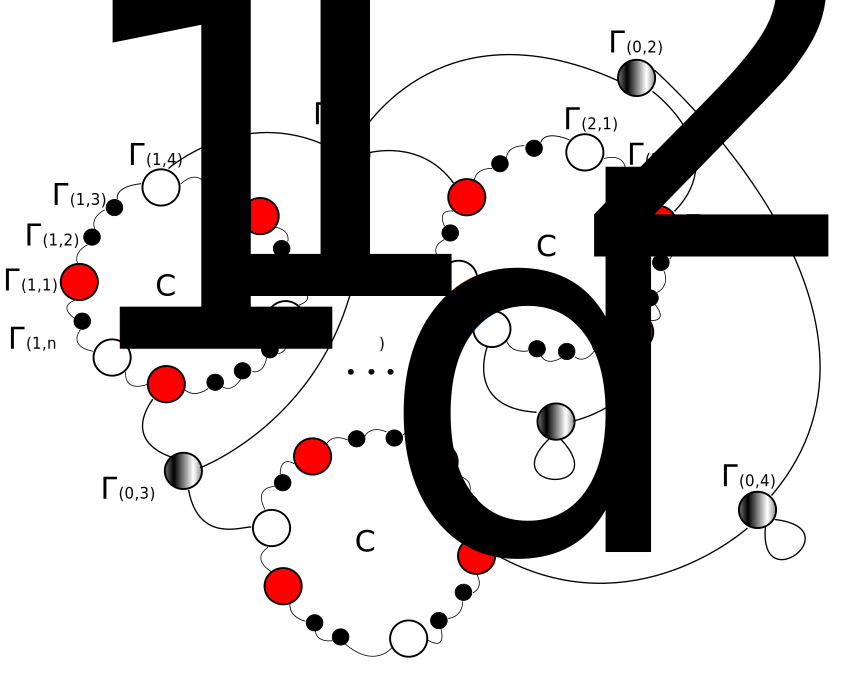
\includegraphics[scale=0.5]{GraphScheme3.png} 
\caption{Класс графов переходов (Шаг 3)}
\label{GraphSchemeTree}
\end{figure}
\end{enumerate}

Стоит отметить, что шаг $3$ может повторяться неоднократно, но конечное число раз.
 
Последнее требование, которое будет наложено заключается в следующем. Изо всех выходных вершин кластеров должны выходить ровно два ребра, ровно как во входные вершины кластеров должно входить также ровно два ребра; что касается сторонних вершин, то и из любой сторонней вершины должны выходить также по два ребра.
















\subsection{Кибернетический подход к изучению систем массового обслуживания с управлением}
Теперь перейдем к описанию основного метода, используемого в данной работе для исследования построенной модели. Не вдаваясь в данном разделе в математические детали, сформулируем основную задачу теории массового обслуживания и некоторые наиболее известные подходы к ее решению. 

Математической моделью системы обслуживания, как правило, является случайный процесс $\brrr{\xi(t) \colon t \in T}$ такой, что случайная величина $\xi(t)$ задает состояние системы в момент $t \in T$. Задача исследовтеля заключается в том, чтобы восстановить по физическому описанию системы вероятностное распределение этого процесса и изучить свойства распределения. Обозримость решения этой задачи во многом зависит от выбора описания состояния системы. В классических работах по данной тематике, например, изучались длина очереди, время ожидания начала обслуживания произвольного требования, число занятых линий. В связи с созданием и развитием А.А.~Боровковым асимптотических методов анализа в теории массового обслуживания в его работах система описывается трехмерным случайным процессом $\brrr{\eta(t), \nu(t), \zeta(t)\colon t \geqslant 0}$, в котором компоненты $\eta(t)$, $\nu(t)$ и $\zeta(t)$ соответственно определяют число поступивших, число получивших отказ и число обслуженных требований за промежуток $[0;t)$. 

Далее, кроме процесса $\brrr{\xi(t) \colon t \in T}$ рассматривают также процесс $\brrr{u(t) \colon t \in T}$, интерпретируемый как управление системой обслуживания. Управление может быть и случайным элементом, и детерменированной величиной. Ограничения на множество всех допустимых управлений имеют различную природу: математическую (например, измеримость), физическую (например, непрерывность), специфика задачи (например, в задачах о назначении приоритетов при обслуживании разнотипных требований).

Таким образом, математик -- исследователь управляемой системы массового обслуживания должен решать непростую задачу по описанию управляемого случайного процесса $\brrr{(\xi(t), u(t)) \colon t \in T}$. Упомянутые подходы обладают тем недостатком, существенно затрудняющими их применение для реальных систем, что достигаемая ими математическая общность не дает возможности принять в расчет многие физические особенности конкретных систем и построить конечномерные распределения рассматриваемого случайного процесса $\brrr{(\xi(t), u(t)) \colon t \in T}$.

В связи с вышесказанным, в данной работе будет применен другой подход, который с единых позиций рассматривает любую управляемую систему. Этот подход называется кибернетическим. Он базируется на трех постулатах. Во--первых, система массового обслуживания, как и многие другие кибернетические системы, функционирует в дискретном времени. Действительно, моменты поступления требований, моменты окончания обслуживания и другие события образуют дискретную совокупность точек на временной оси. Поэтому следует в первую очередь выбрать дискретную временную шкалу $T=\brrr{\tau_0, \tau_1, \ldots}$ и привязывать к ней все другие рассматриваемые величины и объекты. 

Во--вторых, описание состояния элементов системы в любой момент времени $t \geqslant 0$ даже для простых законов распределения входных потоков и длительностей обслуживания приводит к сложным математическим проблемам. Локальный принцип не учитывает в полной мере физическую природу процесса обслуживания и такие важные возможности и особенности действующих систем, как функции ориентации и переналадок, неоднородность требований, изменчивость с течением времени вероятностной структуры входных потоков и длительностей обслуживания, адаптивность логической структуры обслуживающего устройства, наконец, конфликтность ситуаций в управлении и обслуживании. Итак, описание поэлементного строения системы должно быть нелокальным.

В--третьих, следует выбрать уровень детализации, на котором рассматривается система. Исторически первым был метод анализа и синтеза. Сложная система мысленно расчленялась на свои составляющие и каждая часть изучалась отдельно во всей своей полноте. Затем знание обо всех частях соединялось, синтезировалось в знание обо всей совокупности, объединенной в систему. Проблемы, возникающие при таком подходе, уже обсуждались выше. Это и огромное число составляющих, и невозможность полного описания одной части без учета ее взаимодействия с другими частями. Другой подход, появившийся лишь в $\mathrm{\Rmnum{20}}$ веке, носит название <<черный ящик>>. Исследователь вовсе не интересуется устройством системы, а пытается лишь подобрать зависимость <<выхода>> системы от ее <<входа>>. Напротив, кибернетический подход отдает дань умеренности. Считается, что каждая управляемая система обладает схемой, на которой присутствуют элементы небольшого числа типов: 1) внешняя среда, 2) полюса --- точки взаимодействия системы со средой, 3) внешняя и внутренняя память, 4) устройства по переработке информации во внешней и внутренней памяти. Память состоит из ячеек с дискретным множеством состояний. Информацией является совокупность состояний всех ячеек памяти в данный момент времени. Расположение элементов на схеме описывают координаты. Благодаря им система может воздействовать на саму себя в соответствии со своими функциональными свойствами. Функция системы определяет поведение системы массового обслуживания. Она указывает то действие, которое система может совершать, переходя к следующему моменту времени. Таким образом, под состоянием $\xi(\tau)$ системы можно понимать состояния указанных элементов в момент времени $\tau \in T$, и требуется формализовать функцию системы путем совместного рассмотрения поэлементного строения системы и ее функционирования во времени. 

Более подробно и применительно к рассматриваемой задаче кибернетический подход будет описан в следующих разделах. Будет построена математическая модель управляемой системы массового обслуживания в виде счетных управляемых марковских цепей.

















Все рассматриваемые в этой работе случайные элементы определяются на общем вероятностном пространстве $\br{\Omega, {\cal F}, P}$ элементарных исходов $\omega \in \Omega$ с вероятностной мерой $P(A)$, $A \in {\cal F}$, на $\sigma$-алгебре ${\cal F}$. 

Введем следующие случайные величины и элементы, $j \in \brrr{1,2,3,4}$:
\begin{itemize}
\item количество $\vk_{j,i} \in Z_+ $ требований в очереди $O_j$ в момент времени $\tau_i$;
\item состояние обслуживающего устройства $\G_i\in \G = \brrr{\G^{(1)},\G^{(2)}, \ldots, \G^{(n)}}$ в течение времени $\left(\tau_{i-1};\tau_i\right]$;
\item количество $\eta_{j,i}$ требований, поступивших в очередь $O_j$ по потоку $\Pi_j$ в течение времени $\left(\tau_{i};\tau_{i+1}\right]$;
\item количество $\xi_{j,i}$ требований по потоку насыщения $\Pi^{\mathrm{sat}}_j$ в течение времени $\left(\tau_{i};\tau_{i+1}\right]$;
\item количество $\overline{\xi}_{j,i}$ реально обслуженных требований по потоку $\Pi_j$ в течение времени $\left(\tau_{i};\tau_{i+1}\right]$.
\end{itemize}

Тогда для $j \in \brrr{1,2,3}$ имеем
\begin{equation}
\G_{i+1}=h(\G_i,\vk_{3,i}),\quad \vk_{j,i+1}=\max{\brrr{0,\vk_{j,i}+\eta_{j,i}-\xi_{j,i}}}, \quad \overline{\xi}_{j,i} = \min{\brrr{\xi_{j,i},\vk_{j,i}+\eta_{j,i}}}
\label{deterministicLawOne}
\end{equation}
и 
\begin{equation}
\eta_{2,i} = \overline{\xi}_{4,i}, \quad \eta_{4,i}=\overline{\xi}_{1,i}, \quad \vk_{4,i+1}=\vk_{4,i} + \overline{\xi}_{1,i} - \overline{\xi}_{4,i}
 \label{deterministicLawTwo}
\end{equation}
Также для определения длительности $T_{i}$ состояния обслуживающего устройства в течение $\left(\tau_{i-1};\tau_i\right]$, удобно ввести функцию $h_T(\cdot,\cdot)$:
\begin{equation}
T_{i+1}=h_T(\G_i,\vk_{3,i})= \Tt{r'},\quad  \text{ где } \ga{r'}=h(\G_i,\vk_{3,i}).
\label{timeLaw}
\end{equation}

Обозначим через $\vp_j(x,t)$, $j\in \brrr{1,3}$, условную вероятность того, что за время $t>0$ по потоку $\Pi_j$ поступит ровно $b\in Z_+$ требований:
\begin{equation}
\P{ \eta_{j,i} = b}{\G_i=\ga{k,r}, \vk_{3,i}=x}=\vp_j(b,h_T (\ga{k,r}, x)).
\end{equation}
Учитывая закон распределения процесса Пуассона и количества требований в пачках, величины $\vp_j(x,t)$ могут быть найдены из соотношений
\begin{equation}
\sum_{x=0}^{\infty} z^x\vp_j(x,t) = \exp\brrr{\la_j t \br{\sum_{b=1}^{\infty} z^b \pi(b,j) -1}}.
\end{equation}

Для потоков насыщения имеем следующие соотношения:
\begin{align}
\P{\xi_{j,i} = 0}{\G_i=\ga{k,r}, \vk_{3,i} = x} = 1, &\quad \G_{i+1} \notin~^j\G,\\
\P{\xi_{j,i} = \ell_{r',j}}{\G_i=\ga{k,r}, \vk_{3,i} = x} = 1, &\quad \G_{i+1}=\ga{r'}\in~^j\G,
\end{align}
где $j\in \{1, 2, 3\}$, $x \in Z_+$.


Введем для $0 < u \leqslant 1$ и $0 \leqslant k \leqslant x$ величину
\begin{equation}
\psi\br{k,x,u} = C_x^k u^k (1-u)^{x-k}.
\end{equation}
Поскольку требования из очереди $O_4$ независимо друг от друга с вероятностью $p_{k,r}$ на выходе системы поступают в очередь $O_2$, то количество требований в выходном потоке $\Pi_4^{\mathrm{\text{вых}}}$ определяется по биномиальному закону распределения:
\begin{equation}
\P{\overline{\xi}_{4,i} = b}{ \G_i = \ga{k,r}, \vk_{4,i}=x, \vk_{3,i}=\tilde{x}}=\psi\br{b,x,p_{r'}}, \quad \G_{i+1}=\ga{r'}, \quad 0 \leqslant b \leqslant x.
\end{equation}












































Изучим теперь свойства распределения $P(\cdot)$ построенного вероятностного пространства $(\Omega,{\cal F},P(\cdot))$ и, в частности, убедимся в том, что оно отражает основные характеристики рассматриваемой системы массового обслуживания.

Начнем со связи последовательности $X(\omega)=(X_0(\omega), X_1(\omega),\ldots)$ со случайными величинами из \eqref{functionsOne}, \eqref{functionsTwo}, \eqref{functionsThree}. Поскольку (см. \eqref{ProbabilitiesGeneralOne} и \eqref{ProbabilitiesGeneralTwo}) 
\begin{equation*}
P(X_0(\omega)=a_0) = P_0(\eta_0(\omega_0)=a_0) 
\end{equation*}
и
\mll
{\P{X_n(\omega)=a_n}{X_0(\omega) = a_0, X_1(\omega)=a_1,\ldots, X_{n-1}(\omega)=a_{n-1}} = \\
= P_n(a_0,a_1,\ldots, \{\eta_n(\omega_n)=a_n\}),
}
то условные распределения случайных величин $X_n(\omega)$ и распределения случайных величин $\eta_n(\omega_n)=(\eta_{1,n}(\omega_n),\eta_{2,n}(\omega_n),\eta_{3,n}(\omega_n))$ совпадают, $n\geqslant 0$. Таким, образом, $X_n(\omega)$ можно рассматривать как <<продолжение>> величин $\eta_n(\omega_n)$ на общее вероятностное пространство $(\Omega,{\cal F},P(\cdot))$ с исходных пространств $(\Omega_n,{\cal F}_n,P_n(\omega_0,\omega_1,\ldots,\omega_{n-1},\cdot))$. Тогда определенные в прошлом разделе на качественном уровне величины теперь можно определить формально:
	
\begin{equation}
\begin{aligned}
\eta_{j,n}(\omega) &= X_{j,n}(\omega),\quad \overline{\xi}_{4,0}(\omega)=\eta_{2,0}(\omega), & \quad \G_{i+1}(\omega)&=h(\G_{i}(\omega),\vk_{3,i}(\omega)),\\
\vk_{j,i+1}(\omega)&=\max{\left\{ 0,\vk_{j,i}(\omega)+\eta_{j,i}(\omega) - \xi_{j,i}(\omega)\right\}},& \quad
\xi_{j,i}(\omega)&=f_{\xi_j | \G,\vk_3} (\G_i(\omega),x_{3,i}(\omega)),
\end{aligned}
\label{RandomVariablesOne}
\end{equation}
и
\begin{equation}
\vk_{4,i+1}(\omega)=\vk_{4,i}(\omega)+\eta_{4,i}(\omega -\overline{\xi}_{4,i}(\omega)),\quad
\eta_{4,i}(\omega)=f_{\eta_4| \xi_1, \eta_1, \vk_1} (\xi_{1,i}(\omega),\eta_{1,i}(\omega),\vk_{1,i}(\omega)),
\label{RandomVariablesTwo}
\end{equation}
Где $\G_0=\gamma_0=\mathrm{const}$ и $\vk_0=(\vk_{1,0},\vk_{2,0},\vk_{3,0},\vk_{4,0})=(x_{1,0},x_{2,0},x_{3,0},x_{4,0})=\mathrm{const}$.
Величины, определенные в \eqref{RandomVariablesOne} и \eqref{RandomVariablesTwo}, являются случайными величинами, поскольку выражаются через конечное число случайных величин $X_{j,n}(\omega)$, $j\in\{1,2,3\}$, $n\geqslant 0$. Причем 
\mll
{
\P{\eta_{j,n}(\omega)=a_{j,n}}{\eta_{0}(\omega)=a_0,\eta_{1}(\omega)=a_1,\ldots, \eta_{n-1}(\omega)=a_{n-1}} =\\ = \P{X_{j,n}(\omega)=a_{j,n}}{X_0(\omega) = a_0, X_1(\omega)=a_1,\ldots, X_{n-1}(\omega)=a_{n-1}} =\\= \vp_j(a_{j,n},h_T(\G_n(\omega),\vk_{3,n}(\omega)))
}
для $j\in\{1,3\}$ и 
\mll
{
\P{\eta_{2,n}(\omega)=a_{2,n}}{\eta_{0}(\omega)=a_0,\eta_{1}(\omega)=a_1,\ldots, \eta_{n-1}(\omega)=a_{n-1}} =\\ = \P{X_{2,n}(\omega)=a_{2,n}}{X_0(\omega) = a_0, X_1(\omega)=a_1,\ldots, X_{n-1}(\omega)=a_{n-1}} =\\= \begin{cases} \binom{x}{a} p_{k,r}^a(1-p_{k,r})^{x-a}, \quad &\text{если } h(\G_n(\omega),\vk_{3,n}(\omega))=\ga{k,r}, \vk_{4,n}(\omega)=x \\ 0, \quad &\text{иначе}\end{cases}
}
что соответствует вероятностным предпосылкам, заложенным в описание рассматриваемой системы массового обслуживания.
%Учитывая \eqref{probabilitiesTwo}, распишем
%\ml
%{
%P_{n+1}(\omega_0,\omega_1,\ldots,\omega_n,\brrr{\eta_{1,n+1}(\omega_{n+1}) = a_1}) = P_{n+1}(\omega_0,\omega_1,\ldots,\omega_n,\brrr{\omega_{1,n+1} = a_1})=\\
%= \sum_{a_2,a_3 \in Z_+}P_{n+1}(\omega_0,\omega_1,\ldots,\omega_n,\brrr{(\omega_{1,n+1},\omega_{2,n+1},\omega_{3,n+1}) = (a_1,a_2,a_3)})
%}
%

%В первую очередь, определим, чему соответствует последовательность $X(\omega)=\br{X_1(\omega),X_2(\omega),\ldots}$. 


